\documentclass[12pt,letterpaper]{article}
\usepackage{fullpage}
\usepackage[top=2cm, bottom=4.5cm, left=2.5cm, right=2.5cm]{geometry}
\usepackage{amsmath,amsthm,amsfonts,amssymb,amscd}
\usepackage{lastpage}
\usepackage{enumerate}
\usepackage{fancyhdr}
\usepackage{mathrsfs}
\usepackage{xcolor}
\usepackage{graphicx}
\usepackage{listings}
\usepackage{hyperref}

\hypersetup{%
  colorlinks=true,
  linkcolor=blue,
  linkbordercolor={0 0 1}
}
 
\renewcommand\lstlistingname{Algorithm}
\renewcommand\lstlistlistingname{Algorithms}
\def\lstlistingautorefname{Alg.}

\lstdefinestyle{Python}{
    language        = Python,
    frame           = lines, 
    basicstyle      = \footnotesize,
    keywordstyle    = \color{blue},
    stringstyle     = \color{green},
    commentstyle    = \color{red}\ttfamily
}

\lstdefinestyle{Bash}{
   basicstyle=\footnotesize,
   stringstyle=\color{red},
   keywordstyle=\color{blue},
   commentstyle=\color{darkgrey}\slshape,
   morekeywords={linestyle,linetype,linewidth,linecolor,pointtype,nohidden3d,hidden3d,palette,lt,lw,lc,pt,ps,fd,fill,fs,ls},
   framexleftmargin=1mm, framextopmargin=1mm, frame=single
 }
 
 \lstdefinestyle{BBash}{
   backgroundcolor=\color{lightgray},
   basicstyle=\footnotesize,
   stringstyle=\color{red},
   keywordstyle=\color{blue},
   commentstyle=\color{darkgrey}\slshape,
   morekeywords={linestyle,linetype,linewidth,linecolor,pointtype,nohidden3d,hidden3d,palette,lt,lw,lc,pt,ps,fd,fill,fs,ls},
   framexleftmargin=1mm, framextopmargin=1mm, frame=single
 }

\lstdefinestyle{C++}{
    language        = C++,
    frame           = lines, 
    basicstyle      = \footnotesize,
    keywordstyle    = \color{blue},
    stringstyle     = \color{green},
    commentstyle    = \color{red}\ttfamily
}


\pagestyle{fancyplain}
\headheight 35pt

\chead{\textbf{\Large ExaHyPE 2 Tutorial}}
\rhead{ \today}
\cfoot{}
\rfoot{\small\thepage}
\headsep 1.5em

\begin{document}

\begin{figure}[!h]
\centering

\includegraphics[width=0.5\linewidth]{pictures/ExaHyPE_Logo.jpg}
\end{figure}

\section{Introduction}
\label{sec:Introduction}

\vspace{0.2cm}

This document is meant to be an introductory tutorial into ExaHyPE 2. ExaHyPE 2 is part of \textbf{Peano4}, which is an open source framework for solvers on dynamically adaptive Cartesian meshes that was developed by Tobias Weinzierl, who is at the time of writing Professor at the department of Computer Science of Durham University in the United Kingdom.\\ \\
\textbf{ExaHyPE} itself is a hyperbolic PDE engine, the goal of ExaHyPE is to provide a generic engine in which users can implement the specifics of their hyperbolic PDEs and have those be solved by the engine. This is what we will endeavor to do in the following. \\
ExaHyPE solves partial differential equations of the following form:


\begin{equation*}
    \frac{\partial Q}{\partial t} + \nabla . F(Q, \nabla Q) + B(Q) . \nabla Q= S(Q) + \sum_{i = 1}^{n_{ps}} \delta_i
\end{equation*}
\\

This document assumes a succesful installation and configuration of Peano4. \\
Information about how to install and configure Peano4 can be found at \hyperlink{http://www.peano-framework.org/peano/p4/cookbook.pdf}{http://www.peano-framework.org/peano/p4/cookbook.pdf}. Note that the configuration flags "\textit{--enable-ExaHyPE --enable-blockstructured --enable-loadbalancing}" must be set in order to use ExaHyPE 2. \\ 
This document also assumes basic knowledge of Python and C++, as ExaHyPE 2 configuration files are in a python format and the implementation of the functions specific to the PDE are done C++.  \\

\vspace{\fill}

\textbf{Acknowledgments}:
ExaHyPE 2 is the follow-up development of the ExaHyPE project which has been funded
by the EU from 2015–2019.\\
Thank you to Tobias Weinzierl, who is as mentioned above the main programmer not only of Peano4, but also of ExaHyPE 2. Thank you as well to Derek Aguiar, whose template was used in making this document.


\section{Verifying the installation and building a project}
\label{Verifying_and_building}

\vspace{0.2cm}

As mentioned above, we assume a working installation of Peano 4 for this tutorial. Nonetheless we will verify that there are no issues with your installation and show you how to run an ExaHyPE 2 application.\\
First of all, navigate to the folder containing the example scripts in your terminal, this folder is contained in the main Peano4 directory, in the subdirectory "\textit{/examples/ExaHyPE2/ExaHyPE2\_Tutorial}"\\

\begin{lstlisting}[style = Bash]
cd path_to_peano4/examples/ExaHyPE2/ExaHyPE2_Tutorial
\end{lstlisting}

from here we will attempt to assemble our first application by running the following command:

\begin{lstlisting}[style = Bash]
python3 example_scripts/euler2D.py
\end{lstlisting}

If at this point you receive the following error message:
\textbf{ModuleNotFoundError: No module named 'peano4'} this means you have not properly included the required python path, you can do this by running the following command and then reattempting the assembly as above.

\begin{lstlisting}[style = Bash]
export PYTHONPATH=../../../Peano/python
\end{lstlisting}

If this still does not work, you may have improperly configured your installation of Peano 4, refer to the \hyperlink{http://www.peano-framework.org/peano/p4/cookbook.pdf}{Peano cookbook} for instructions on how to re-configure and re-build Peano 4, and don't forget to add at least the configuration flags: "\textit{--enable-ExaHyPE --enable-blockstructured --enable-loadbalancing}". Then, repeat the steps above.\\

Hopefully you should at this point have succesfully compiled your application. If you have you should see a number of files have appeared in your working directory. We will ignore most of these for now, but know that these contain the implementation of the ExaHyPE 2 simulation.\\
One file in particular is of interest to us now: the file simply named Euler2D is the executable for our implementation. We will therefore run this executable file by using the following command:

\begin{lstlisting}[style = Bash]
./Euler2D
\end{lstlisting}

which should hopefully run succesfully, as you can verify by the appearance of a number of files with the prefix: "\textbf{solution-euler2D}". These contain the solution of our problem, which we will take a look at as soon as we have an understanding of how our problem is defined.\newpage

\section{Our first Configuration file}
\label{section_3}


We should now have executed our first ExaHyPE 2 application, but in order to understand what it is that we have executed, let us take a look at the file which defined this application: \textbf{euler2D.py}\\
As mentioned in the \hyperref[sec:Introduction]{Introduction}, the configuration files are in python, so it should surprise noone that they start with the following:

\begin{lstlisting}[style = Python]
import peano4
import ExaHyPE2
\end{lstlisting}

These merely import the necessary packages from Peano4 and ExaHyPE 2 which will let us define and build our project. Speaking of defining our project, this happens in the next step:\\

\begin{lstlisting}[style = Python]
project = ExaHyPE2.Project( ["examples", "ExaHyPE2", "euler2D"],
                             "euler2D", ".", executable="Euler2D" )
\end{lstlisting}

Next we will define and add a solver to this project:\\

\begin{lstlisting}[style = Python]
thesolver = ExaHyPE2.solvers.fv.rusanov.GlobalFixedTimeStep(
  name="euler2D",
  patch_size=3,
  unknowns=4, auxiliary_variables=0,
  min_volume_h=0.01, max_volume_h=0.01,
  time_step_size=0.001,
  flux = ExaHyPE2.solvers.fv.PDETerms.User_Defined_Implementation
)
\end{lstlisting}

most of this should be self-explanatory and some pieces will be explained in more detail later, but a few things deserve special mention here.\\
First is the solver itself, the type \textit{ExaHyPE2.solvers.fv.rusanov.GlobalFixedTimeStep()} indicates the type of solver. There are a number of solvers available but in this case for simplicity's sake we have chosen a finite volume, rusanov solver with global fixed timestep.\\
For the parameters of this solver: "\textit{name="euler2D"}", this defines the name of the project and therefore of the files generated by ExaHyPE 2 that will help define the application. "\textit{unknowns=4}" and "\textit{auxiliary\_variables=0}" define the variables of our equation, in this case we have a partial differential equation with 4 component variables but no auxiliary variables.\\ 
The last thing worth mentioning is the parameter \textit{flux} which we have here set to some user defined implementation. We will need to define this in a subsequent step.
\newpage

Next we define the parameters for our simulation, this is where we define the volume of our domain and the number of dimensions for example, but also where basic information about the plotting behaviour is defined:
\begin{lstlisting}[style = Python]
build_mode = peano4.output.CompileMode.Release
project.set_global_simulation_parameters(
  dimensions = 2,
  offset = [0.0,0.0],
  size = [1.0,1.0],
  end_time = 0.01,
  first_plot_time_stamp = 0.0,
  time_in_between_plots = 0.001
)\end{lstlisting}

Finally, given all the information above we can generate and build a working application.

\begin{lstlisting}[style = Python]
project.set_load_balancing( "toolbox::loadbalancing::RecursiveSubdivision", 
            "new ::ExaHyPE2::LoadBalancingConfiguration()" )
project.set_Peano4_installation( "../../../", build_mode )
peano4_project = project.generate_Peano4_project(False)
peano4_project.build(make_clean_first=True, number_of_parallel_builds=4)
)\end{lstlisting}

Logically, this application is still missing some information about the implementation of this PDE. We mentioned that we would need to define the flux, but we have also not yet defined any initial conditions or boundary conditions.\\
We will do so in the next step.

\newpage

\section{Our first implementation file}

The astute reader might have noticed that before we built our project, there were already a few files in the containing folder, most noticeably one that has to do with the project they just built: \textbf{euler2D.cpp}. We will be taking a look at this file next since, as you most likely have already guessed, it contains the implementation of our PDE.
\\ \\
Before we do this however, we will quickly define the PDE that is to come. As the name of the file will have already indicated, this is the 2-dimensional euler equation which, in the finite volume form and given no external forces, appears as follows:

\begin{equation*} \label{Euler_equation}
    \frac{\partial}{\partial t}\left(
    \begin{array}{lr} \rho \\
                      \rho u_1 \\
                      \rho u_2 \\
                      E_t 
                      \end{array} \right) +
    \nabla \begin{pmatrix}
                      \rho u_1          & \rho u_2\\
                      \rho u_1^2 + p    & \rho u_1 u_2 \\
                      \rho u_2 u_1      & \rho u_2^2 + p \\
                      (E_t + p) u_1     & (E_t + p) u_2
    \end{pmatrix}  = \vec{0}
\end{equation*}

where $\rho$ is the density, $u$ is the velocity, $E_t$ is the energy and $p$ is the pressure.\\
In order to implement this equation, four things are needed: the initial condition, the boundary conditions, the maximal eigenvalue and the flux.\\

We start with the initial conditions: here we define a starting configuration with a uniform density of \textbf{0.1}, a uniform starting momentum of \textbf{0.0} in both x and y directions and a starting energy that is \textbf{1.0} on the left half of the domain and \textbf{0.0} on the right half of the domain. Note that we use momentums and not velocities as our variables of choice, this will affect the formulation of some of the equations later.\\

\begin{lstlisting}[style = C++]
void examples::ExaHyPE2::euler2D::euler2D::initialCondition(
  double * __restrict__ Q,
  const tarch::la::Vector<Dimensions,double>&  volumeCentre,
  const tarch::la::Vector<Dimensions,double>&  volumeH,
  bool                                         gridIsConstructred
) {

	Q[0] = 0.1;                         // density
	Q[1] = 0.0;                         // momentum in x direction
        Q[2] = 0.0;                         // momentum in y direction
  
	bool isLeft = (volumeCentre[0]<0.5);
	Q[3] = (isLeft ? 1.0 : 0.0);        //energy
}
\end{lstlisting}

\newpage

Next we can define the largest eigenvalue of our system. This is important because it defines a lot of the behaviour of the PDE, and among others the maximum allowable timestep for which a lot of solvers remain stable. The eigenvalues of the 2 dimensional euler equation are:

\begin{equation*}
    \left(
    \begin{array}{lr} \lambda_1 \\
                      \lambda_2 \\
                      \lambda_3
                      \end{array} \right) =
    \left(
    \begin{array}{lr} u - c \\
                      u \\
                      u + c
                      \end{array} \right)
\end{equation*}

where $c$ is the wave propagation speed. For an ideal gas, c depends on the pressure as follows:

\begin{equation*}
    \left(
    \begin{array}{lr} c \\
                      p
                      \end{array} \right) =
    \left(
    \begin{array}{lr} \sqrt[]{\frac{\gamma  p}{\rho}} \\
                      (\gamma - 1) ( E_t - \frac{1}{2 \rho} (\rho u)^2 ) 
                      \end{array} \right)
\end{equation*}

which we can combine to give the following function for the maximal eigenvalue:

\begin{lstlisting}[style = C++]
double ::examples::ExaHyPE2::euler2D::euler2D::maxEigenvalue(
  const double * __restrict__ Q, // Q[4+0],
  const tarch::la::Vector<Dimensions,double>&  faceCentre,
  const tarch::la::Vector<Dimensions,double>&  volumeH,
  double                                       t,
  int                                          normal
)  {
	  const double irho = 1.0/Q[0];
	  // based on the assumption that the fluid is an ideal gas
	  const double gamma = 1.4;  //gamma chosen for dry air
	  const double p = (gamma-1) * (Q[3] - 0.5*irho*(Q[1]*Q[1]+Q[2]*Q[2]));
	  const double c   = std::sqrt(gamma * p * irho);

	  double result = 1.0;
	  switch(normal){
	  case 0: //x
		  result = std::max( std::abs(Q[1] * irho - c),
		        std::abs(Q[1] * irho + c) );
		  break;
	  case 1: //y
		  result = std::max( std::abs(Q[2] * irho - c),
		        std::abs(Q[2] * irho + c) );
		  break;
	  }
	  return result;
}
\end{lstlisting}

Notice that we compute the result twice depending on the function parameter normal. This parameter defines which direction we are computing the eigenvalue in. This will in turn define which velocity we use. We will do a similar trick when computing the fluxes, where it might be more intuitively clear that the flux in x and y direction need not be the same. \\

Next, let's define our flux in x and y direction according to our \hyperref[Euler_equation]{previous definition}.
As with the eigenvalues, the directions of the flux are defined by the normal parameter. This parameter defines through which surface, and therefore in which direction, the flux is being computed. Here if the normal is \textbf{0}, we are computing the flux in x direction and if the normal is \textbf{1}, we are computing the flux in y direction. For higher dimensions, there would logically be additional directions to implement the flux in.

Our fluxes in x and y directions are:

\begin{equation*}
    F_x = \begin{pmatrix}
                      \rho u_1      \\
                      \rho u_1^2 + p\\
                      \rho u_2 u_1  \\
                      (E_t + p) u_1 
    \end{pmatrix}, \hspace{\fill} 
    F_y =\begin{pmatrix}
                      \rho u_2\\
                      \rho u_1 u_2 \\
                      \rho u_2^2 + p \\
                      (E_t + p) u_2
    \end{pmatrix}
\end{equation*}\\

Which we implement as:

\begin{lstlisting}[style = C++]
void ::examples::ExaHyPE2::euler2D::euler2D::flux(
  const double * __restrict__ Q, // Q[4+0],
  const tarch::la::Vector<Dimensions,double>&  faceCentre,
  const tarch::la::Vector<Dimensions,double>&  volumeH,
  double                                       t,
  int                                          normal,
  double * __restrict__ F // F[4]
)  {
  const double irho = 1.0/Q[0];
  // based on the assumption that the fluid is an ideal gas
  const double gamma = 1.4; //gamma chosen for dry air
  const double p = (gamma-1) * (Q[3] - 0.5*irho*(Q[1]*Q[1]+Q[2]*Q[2]));
  
  switch(normal){  
  case 0: //in x direction
	  F[0] = Q[1];                    //density
	  F[1] = irho * Q[1] * Q[1] + p;  //velocity in x direction 
	  F[2] = irho * Q[1] * Q[2];      //velocity in y direction
	  F[3] = irho * Q[1] *(Q[3] + p); //energy
	  break;
  case 1: //in y direction
	  F[0] = Q[2];                    //density
	  F[1] = irho * Q[2] * Q[1];      //velocity in x direction
	  F[2] = irho * Q[2] * Q[2] + p;  //velocity in y direction
	  F[3] = irho * Q[2] *(Q[3] + p); //energy
	  break;
  }  
}
\end{lstlisting}

\newpage

Finally, we can define our boundary conditions. For this simple case, we will simply use absorbing boundary conditions on everything but the density. This means all values except the density will be zero on the boundary and the density will be the same inside as outside of the boundary.\\ \\


\begin{lstlisting}[style = C++]
void examples::ExaHyPE2::euler2D::euler2D::boundaryConditions(
  const double * __restrict__                  Qinside, // Qinside[4+0]
  double * __restrict__                        Qoutside, // Qoutside[4+0]
  const tarch::la::Vector<Dimensions,double>&  faceCentre,
  const tarch::la::Vector<Dimensions,double>&  volumeH,
  double                                       t,
  int                                          normal
) {
  
  Qoutside[0] = Qinside[0]; //density
  Qoutside[1] = 0;	    //velocity in x direction
  Qoutside[2] = 0;	    //velocity in y direction
  Qoutside[3] = 0;	    //Energy
  
}
\end{lstlisting}


And that is all there is to it, all that was needed was one file defining our problem and four small functions defining how to compute it. \\
But now that we have computed our problem, we'd like to visualize it.\\
We will do so in the next (very short) section.

\newpage

\section{Visualizing results from ExaHyPE}
\label{Visualize}

\vspace{0.3cm}

Peano 4 and therefore ExaHyPE per default write the results in a native format. These are defined by two files, a more general one called \textbf{solution-\textit{project\_name}.peano-patch-file} and individual ones for each logged time step called \textbf{solution-\textit{p}-\textit{file\_number}-rank-\textit{rank\_number}.peano-patch-file}.\\
The first of these two just contains information linking each file of the second type to a specific timestamp, it allows an interpreter to find the other files and assign them to the proper location and time. The second type contains the values computed in each patch as an array which contains one after another the values of each variable for each cell in the patch. The patches are specified by their position and size.\\
This relatively simple, machine readable format allows one to easily create applications for processing and visualising these results oneself. A few of these are provided with Peano 4 as is (see the \hyperlink{http://www.peano-framework.org/peano/p4/cookbook.pdf}{cookbook, appendix B}).

In our case, we will just mention how to convert these to VTU format, which would allow one to read them with paraview for example, the most commonly used application for scientific visualization.
To do so, simply use the command:
\begin{lstlisting}[style = Bash]
pvpython path_to_peano4/python/peano4/visualization/render.py \
solution-project_name.peano-patch-file
\end{lstlisting}
with the corresponding path to the Peano 4 installation directory and project name. In the case of our previous example, this would be:
\begin{lstlisting}[style = Bash]
pvpython ../../../python/peano4/visualization/render.py \
 solution-euler2D.peano-patch-file
\end{lstlisting}
For our aforementioned example, this provides following results for the energy at the start and end of the computed time:

\begin{figure}[!h]
\centering
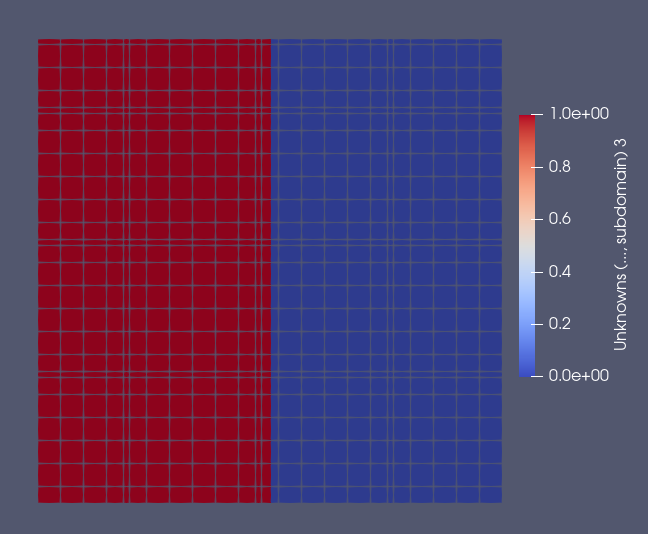
\includegraphics[width=0.40\linewidth]{pictures/euler2D_start.png}
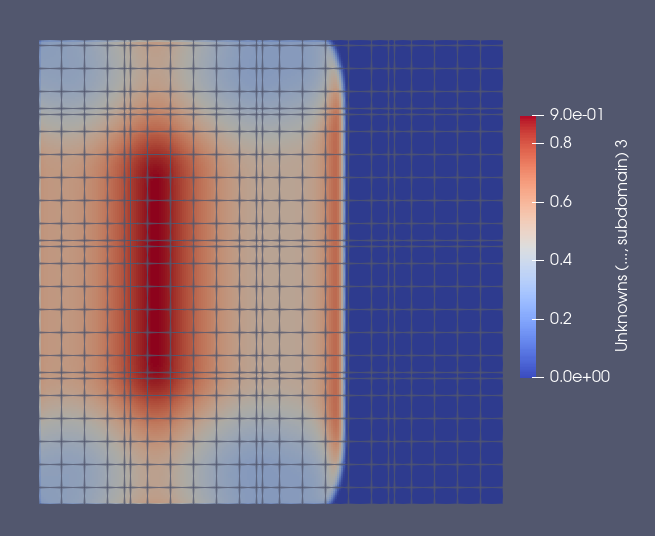
\includegraphics[width=0.40\linewidth]{pictures/euler2D_end.png}
\caption{The computed energy of the Euler equations respectively at time t=0.0 and t=1.0}
\end{figure}

\newpage

\section{Our first exercice}
\vspace{0.2cm}

Now that we have an example of how to implement an equation, we will start by attempting to implement this same equation in three dimensions. The three-dimensional Euler equation appears as follows:

\begin{equation*}
    \frac{\partial}{\partial t}\left(
        \begin{array}{lr}
                    \rho \\
                    \rho u_1 \\
                    \rho u_2 \\
                    \rho u_3 \\
                    E_t 
        \end{array} \right) +
    \nabla
        \begin{pmatrix}
            \rho u_1          & \rho u_2            & \rho u_3\\
            \rho u_1^2 + p    & \rho u_1 u_2        & \rho u_1 u_3 \\
            \rho u_2 u_1      & \rho u_2^2 + p      & \rho u_2 u_3 \\
            \rho u_3 u_1      & \rho u_3 u_2 + p    & \rho u_3^2 + p \\
            (E_t + p) u_1     & (E_t + p) u_2       & (E_t + p) u_3
        \end{pmatrix}  = \vec{0}
\end{equation*}

This has the same eigenvalues as the 2D solution:
\begin{equation*}
    \lambda = \left( \begin{array}{lr}
                     c \\
                     0 \\
                    -c \\
        \end{array} \right)
\end{equation*}

And you can use the same approximation for the pressure and wave velocity:
\begin{equation*}
    \left( \begin{array}{lr}
            \gamma \\ 
            p \\ 
            c \end{array} \right) =
    \left( \begin{array}{lr}
                     1.4 \\
                     (\gamma - 1) * ( E_t - \frac{\rho \|u\|}{2} ) \\
                    -c \\
        \end{array} \right)
\end{equation*}

\begin{enumerate}
    \item     
        First, look at the specification file \textbf{Euler3D.py} in the directory \textit{example-scripts}. It is currently an (almost) exact copy of \textbf{Euler2D.py}.\\
        You will need to change the total number of variables as well as the domain boundaries in order to simulate the problem in three dimensions.
    \item
        Second, build the project. If you have forgotten how to do this, refer to \hyperref[Verifying_and_building]{the first section}.\\
        
        Once your project has been built, you will need to implement the functions in the new file \textbf{euler3D.cpp}. You can take inspiration for this from \textbf{euler2d.cpp}.
    \item
        Start by defining the initial conditions. For this, we want the initial density to be \textbf{0.1} everywhere, the initial velocities to be \textbf{0.0} everywhere and the initial energy to be \textbf{1} in a radius of \textbf{0.05} around the center of the domain, and \textbf{0.0} anywhere else.\\
        (Hint: use the function \textit{tarch::la::norm2()} to compute the norm of a vector)
    \item
        Next, fill in the maximal eigenvalue and the boundary conditions. For boundary conditions, you can once again choose absorbing boundary conditions for all but the density, this means all values except for the density should be \textbf{0.0} at the boundary, and the density should be the same as inside of the domain.
    \item
        Finally, fill in the flux.
    \item
        Once you've done all of this, rebuild the program (Hint: you can just use the command \textbf{make} if you haven't made any modifications to the configuration file.)\\ Then execute the program (this may take a little while, there is quite a lot of computation to be done now), convert the files to a readable format (\hyperref[Visualize]{see the previous section}) and take a look. Congratulations, you've implemented your first PDE in ExaHyPE 2!
\end{enumerate}

If at any time you are stuck and incapable of finding an answer, a solution is provided in the directory \textbf{example\_solutions}.

\begin{figure}[!h]
\centering
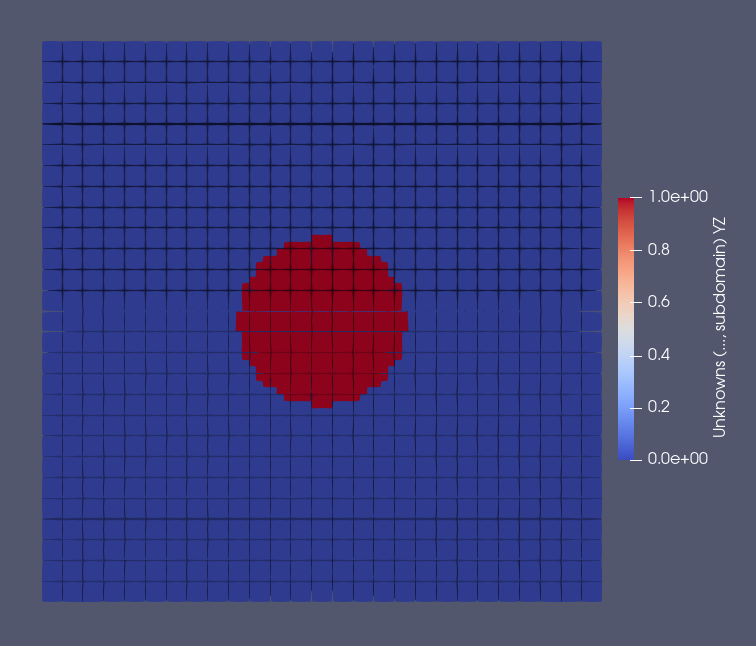
\includegraphics[width=0.40\linewidth]{pictures/euler3D_start.png}
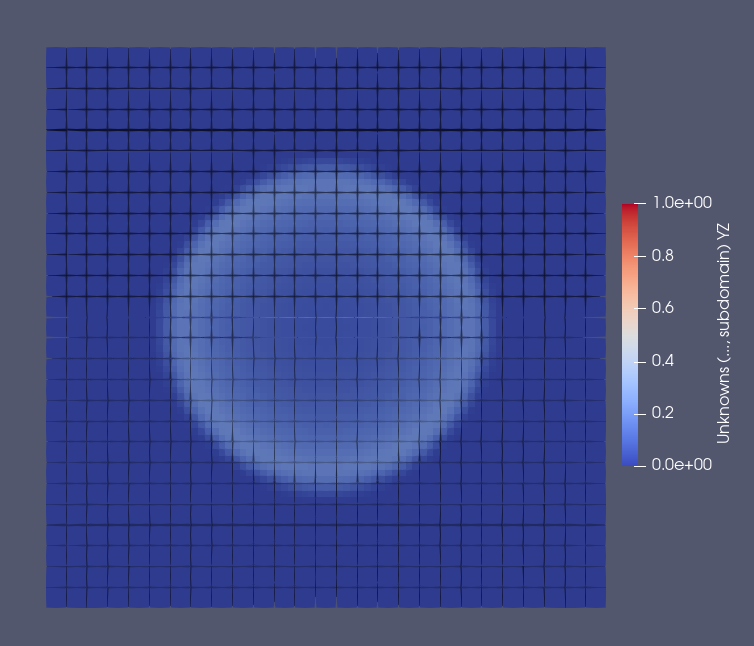
\includegraphics[width=0.40\linewidth]{pictures/euler3D_end.png}
\caption{The computed energy of the 3D Euler equations at times t=0.0 and t=1.0}
\end{figure}

\newpage

\section{Mesh width and mesh refinement}
\label{refinement}

\vspace{0.2cm}

If you've completed the previous exercice, you may have noticed that it's runtime was quite a bit longer than that of the first example. This is true even though the width of the cells was reduced from 243 by dimension to 81 by dimension. Nonetheless, going from two to three dimensions means the total number of cells increased from $243*243=59049$ to $81*81*81=531441$. In addition to this, the fluxes need to be computed in an additional dimensions for each cell, which adds complexity as well.\\
All of this means we need to consider our cell size carefully, so in a first step we will discuss how the cell size is calculated. For this, we return to the specification file that we defined in \hyperref[section_3]{section 3}. In particular, we will take another look at the solver definition:\\

\begin{lstlisting}[style = Python]
thesolver = ExaHyPE2.solvers.fv.rusanov.GlobalFixedTimeStep(
  name="euler2D",
  patch_size=3,
  unknowns=4, auxiliary_variables=0,
  min_volume_h=0.01, max_volume_h=0.01,
  time_step_size=0.001,
  flux = ExaHyPE2.solvers.fv.PDETerms.User_Defined_Implementation
)
\end{lstlisting}

The parameter that interests us here is \textbf{max\_volume\_h}. This determines the maximal allowable size for cells in our volume, in essence guaranteeing $max\_volume\_h > cell\_size$.\\
However since Peano is based upon three-partitioning, it refines the domain into $3^d$ cells, where $d$ is the smallest possible integer that satisfies $max\_volume\_h > domain\_size / 3^d$.\\
For our example above, we have set a domain size of $1.0$ in each direction and $max\_volume\_h = 0.01$, this means that there are a total of 243 cells in each dimension.\\
Of these, two are used for the boundary conditions, which means there are a total of 241 cells per dimension inside the domain.\\
This means there are actually a total of $241*241=58081$ cells inside the domain, or (with a parameter \textit{max\_volume\_h=0.03}) $79*79*79=493039$ cells in three dimensions.

In short, if one wishes to increase or decrease the mesh size, one can just modify the parameter $max\_volume\_h$.\\
You may have noticed that there is a second parameter $min\_volume\_h$ however, and this parameter logically determines the minimal mesh size. If this parameter is given a value lower or equal to $max\_volume\_h / 3$ (again, three-partitioning), adaptive refinement is switched on.\\
This adaptive refinement must be defined by adding one additional line to the configuration file however:\\

\begin{lstlisting}[style = Python]
thesolver.set_implementation(
refinement criterion=ExaHyPE2.solvers.fv.PDETerms.User_Defined_Implementation
)
\end{lstlisting}

After building the project with this line added, you will see one additional function in the implementation file:

\begin{lstlisting}[style = C++]
::ExaHyPE2::RefinementCommand examples::ExaHyPE2::euler::euler3D::refinementCriterion(
  const double * __restrict__ Q, // Q[5+0],
  const tarch::la::Vector<Dimensions,double>&  volumeCentre,
  const tarch::la::Vector<Dimensions,double>&  volumeH,
  double                                       t
) { }
\end{lstlisting}

There are three valid return values for this function:

\begin{lstlisting}[style = C++]
::ExaHyPE2::RefinementCommand::Keep
::ExaHyPE2::RefinementCommand::Refine
::ExaHyPE2::RefinementCommand::Coarsen
\end{lstlisting}

which respectively keep, refine or coarsen the mesh refinement for the current cell.\\
In a next step, we will attempt to use these to implement the shallow water equations.

\newpage

\section{Our second exercice}

In this exercice, we will implement the two-dimensional shallow water equations using adaptive refinement.\\
The shallow water equations, which describe the flow of a fluid given the assumption that the horizontal length scale is much higher than the vertical length scale, are defined by following formula:

\begin{equation*} \label{SWE}
    \frac{\partial}{\partial t}\left(
    \begin{array}{lr} h \\
        h u_1 \\
        h u_2 \\
        b 
        \end{array} \right) +
    \nabla \begin{pmatrix}
        h u_1           & h u_2     \\
        h u_1^2         & h u_1 u_2 \\
        h u_2 u_1       & h u_2^2   \\
        0               & 0
    \end{pmatrix} +
    \begin{pmatrix}
        0                     & 0\\
        h g*\partial_x(b+h)   & 0\\
        0                     & h g*\partial_y(b+h) \\
        0                     & 0
    \end{pmatrix}  = \vec{0}
\end{equation*}

With eigenvalues:

\begin{equation*}
    \left(
    \begin{array}{lr}
        \lambda_1 \\
        \lambda_2 \\
        \lambda_3 
    \end{array} \right) =
    \left(
    \begin{array}{lr}
        h u + \sqrt{g (h+b)} \\
        h u \\
        h u - \sqrt{g (h+b)} \\
    \end{array} \right)
\end{equation*}

This depends on the fluid height h, velocities in x and y direction, the bathimetry b (the height of the floor underneath the fluid) and the gravity g. We still have a flux, as with the previous equations but in addition to this we have a third term, which is a non-conservative part (this just means it depends on the spatial derivatives of the considered variables). This was added to our solver like the flux: by adding a user-defined non-conservative term:

\begin{lstlisting}[style = Python]
  ncp = ExaHyPE2.solvers.fv.PDETerms.User_Defined_Implementation
\end{lstlisting}

We also for the first time have an auxiliary variable since the bathimetry never changes. We can define this auxiliary variable by setting the parameter \textit{auxiliary\_variables} in the solver to \textbf{1} instead of \textbf{0}. These auxiliary variables are accessed in the same way as the regular variables, except that they cannot be modified after the initial conditions have been set.\\
Boundary conditions for these auxiliary variables should be defined, but no flux or non-conservative product can be set.

\begin{enumerate}
    \item
        Start by building the project defined by the configuration file \textbf{SWE.py}. If you have forgotten how to do this, refer to \hyperref[Verifying_and_building]{the first section}.\\
        
        Once your project has been built, you will need to implement the functions in the new file \textbf{swe.cpp}.
    \item
        Next, define the initial conditions. For this, we want the initial water height to be \textbf{1.0} everywhere, the initial velocities to be \textbf{0.0} everywhere and the bathimetry should be \textbf{0.0} in a radius of \textbf{0.20} around the center of the domain, and \textbf{0.1} anywhere else.\\
        (Hint: use the function \textit{tarch::la::norm2()} to compute the norm of a vector)
    \item
        Then, fill in the maximal eigenvalue and the boundary conditions. For boundary conditions, you can choose reflecting boundary conditions, this means all values should be the same outside as inside of the boundary.
    \item
        Once this is done, fill in the flux.
    \item
        Next, fill in the non-conservative part. This function has a parameter \textbf{deltaQ} through which you can access the space derivatives of the computed and auxiliary variables in the direction defined by the \textbf{normal}'s current value.
    \item
        Finally, define the refinement. Remember from \hyperref[refinement]{the previous section} that there are three valid return values for this function. For this application, we want a higher refinement where the bathimetry jumps from \textbf{0.0} to \textbf{0.1}.\\
        Refine cells that are within a radius of \textbf{0.19} to \textbf{0.2} from the center of the volume, and coarsen those which are not.
    \item
        Once you've done all of this, regenerate the program (Hint: you can just use the command \textbf{make} if you haven't made any modifications to the configuration file.) Then execute the program (this may take some time), convert the files to a readable format (\hyperref[Visualize]{see here}) and take a look. Notice that the grid is no longer uniform, it has been refined.
\end{enumerate}

\begin{figure}[!h]
\centering
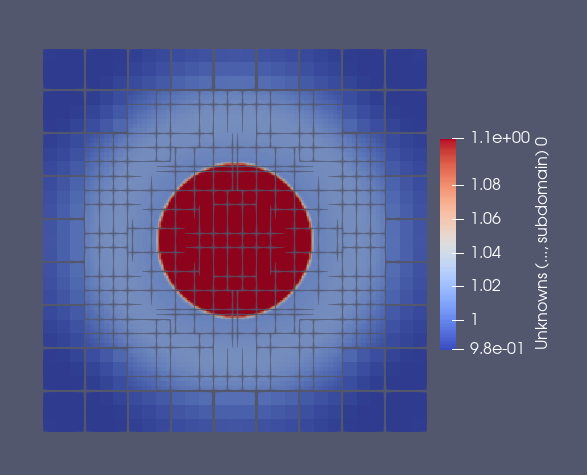
\includegraphics[height=0.50\linewidth]{pictures/SWE_end.png}
\caption{The computed height of the fluid according to our computation of the shallow water equations after 0.2s. The fluid has rushed in from the sides in order to fill the depression at the centre.}
\end{figure}

\end{document}
